\documentclass{handout}

%\SetInstructor{Capt Steven Beyer}
\SetCourseTitle{ECE210: Introduction to Electrical and Computer Engineering}
\SetSemester{Spring 2019}
\SetHandoutTitle{Lab 11 - Obstacle Avoidance}

%\ShowAllBlanks

\usepackage[obeyspaces]{url}
\input{../arduinoLanguage.tex}

%\showsoln \setsolncolor{red}

\lstset { %
	language=Arduino,
	frame=none,
	basicstyle=\footnotesize,
}

\begin{document}
	%	\footnotetext{Examples are abstracted from Tutorials Point, "Arduino", 2019, accessed Feb 18, 2019. [Online]. Available: https://www.tutorialspoint.com/arduino/index.htm}
	\maketitle
	
	\section{Collaboration Policy.}
	This is a team-of-two or individual laboratory. You may use any of the authorized resources listed below. DO NOT copy anyone else’s work.
	
	\textbf{Authorized Resources:} You may use any electronic or hard copy resource at your disposal as long as 1) you cite your sources and 2) your use of the materials does not go against the intent of the assignment. For example, you can use a software library that you find online to help develop a project if you cite where you found it. However, you cannot complete your project by copying all of the source code, schematics, etc and simply running it on the required hardware.
	
	\section{Documentation.}
	\textit{Date:}
	
	\textit{Instructor who helped me:}
	
	\textit{Help received:}
	
	\section{Objectives.} 
	\begin{enumerate}
		\item Become familiar with the Sharp GP2Y0A51SK0F Analog Distance Sensor.
		\item Utilize the Arduino to detect walls.
		\item Integrate the Distance Sensor with the DFECBot and program the DFECBot to avoid obstacles.
	\end{enumerate}
	
	\section{Materials.}
	\begin{enumerate}
		\item 3x Sharp GP2Y0A51SK0F Analog Distance Sensor
		\item 3x 3-pin Female JST Cables
		\item USB Programming Cable
		\item DFECBot
	\end{enumerate}
	
	\newpage
	\clearpage
	\pagebreak
	
	\section{Introduction.}
	
	\subsection{Sharp GP2Y0A51SK0F Analog Distance Sensor}
	The Sharp GP2Y0A51SK0F Analog Distance Sensor uses an infrared radiation (IR) reflectance sensor with an IR light-emitting diode (LED) and an IR sensitive phototransistor.\footnote{GP2Y0A51SK0F Datasheet, \url{https://www.pololu.com/file/0J845/GP2Y0A41SK0F.pdf.pdf}} The sensors will be powered using the $5\ V$ and ground pins on the Arduino. 
	
	Connect your three Distance Sensors to the mounts on the front of the motor layer (Layer B). Secure them using six $\#2-56\ x\ 1/4”$ bolts and nuts. Wire the sensors according to the schematic shown in Figure~\ref{Fig IR}.
	
	\begin{figure} [H]
		\centering
		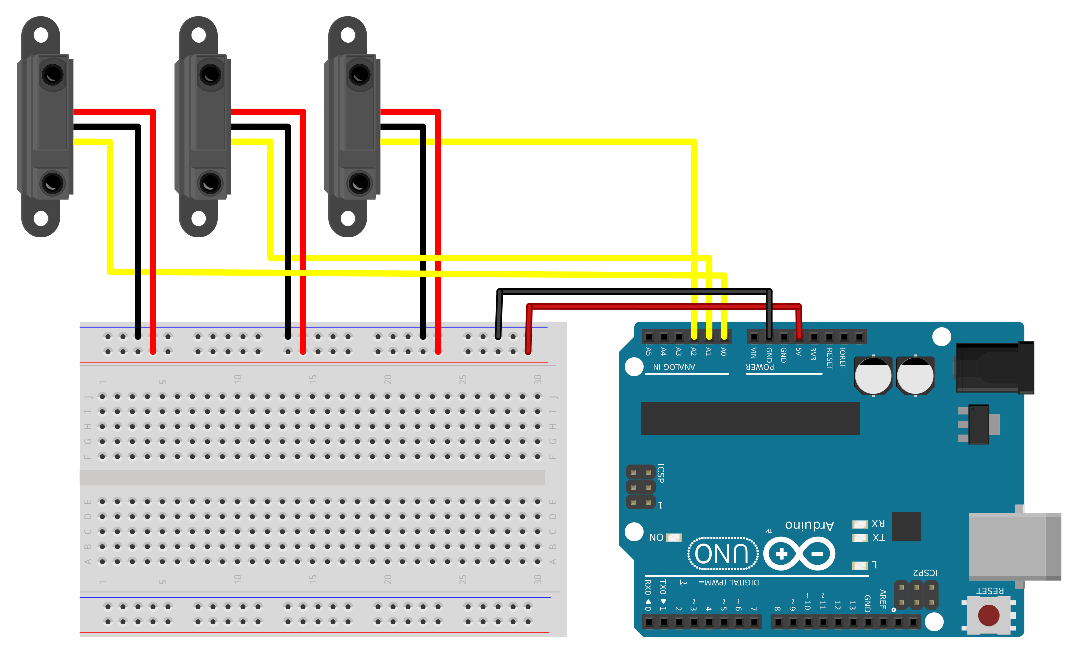
\includegraphics[width=.75\textwidth]{ir.eps}
		\caption{Sharp GP2Y0A51SK0F Analog Distance Sensor Wiring Schematic}
		\label{Fig IR}
	\end{figure}
	
	\subsection{Example Code}
	Browse to \path{K:\DF\DFEC\ECE210\Labs\Lab 11 - Obstacle Avoidance} and copy the \\ \path{robot_obstacleavoidance} folder to your computer. Open \path{robot_obstacleavoidance.ino}. Opening the \textit{.ino} file should open 3 files in your Arduino IDE: \path{robot_obstacleavoidance.ino}, \path{drive.h}, and \path{TB6612FNG.h}. The two \textit{.h} files are the same header files used during previous labs and the \textit{.ino} file is your Arduino sketch.
	
	\subsubsection{robot\_linefollowing.ino}
	This example Arduino Sketch provides code to read the values outputted by the DFECBot's left Distance Sensor (see below example) and convert the value to a distance.
	
	\begin{lstlisting}
		/*
		* Function used to convert from analog voltage to distance. 
		*  Derived from graph in GP2Y0A51SK0F datasheet found at 
		*  https://www.pololu.com/product/2450/resources
		*  The IR sensor is effective between 2-15 cm.
		*/
		float distCalc(float sensorVal){
			return 11.5402*pow(0.995796, sensorVal);
		}
	\end{lstlisting}
	
	\begin{lstlisting}
		// read/convert/print value ouputted by DFECBot's left IR sensor
		float ir_L = analogRead(irL);
		float distL = distCalc(ir_L);
		Serial.print("Left: "); Serial.println(distL);
	\end{lstlisting}
	
	\newpage
	\clearpage
	\pagebreak
	
	\section{Procedure}
	\textbf{Use the example code provided, \path{TB6612FNG.H}, and \path{drive.h} to code the DFECBot to do the following:}
		
	\begin{enumerate}
		\item Print the values from the DFECBot's center and right GP2Y0A51SK0F Analog Distance Sensor to the serial monitor.
		\item Use a ruler to confirm the accuracy of each distance sensor - the sensor should be fairly accurate between $3\ cm$ and $12\ cm$.
		\item Program the DFECBot to detect  an object within $4\ cm$ in front of, to the left of, and to the right of the DFECBott using the three Distance Sensors.
			\begin{enumerate}
				\item Drive forward.
				\item If the front sensor detects an object, randomly turn right or left.
				\item If the front and left sensors detect an object, turn right.
				\item If the front and right sensors detect an object, turn left.
				\item If all three sensors detect an object, turn around.
			\end{enumerate}
				
			\item \textbf{Optional --} Limit drifting within a maze.
				
			\begin{enumerate}
				\item If the left sensor detects an object (within $3\ cm$) and the front sensor does not, turn right slightly until the left sensor does not detect an object.
				\item If the right sensor detects an object (within $3\ cm$) and the front sensor does not, turn left slightly until the right sensor does not detect an object.
			\end{enumerate}
			
			\textbf{Hint:} You may need to use the two functions in \path{drive.h} to make a slight right or left correction.
	\end{enumerate} 	
\end{document}
